%%
% The BIThesis Template for Undergraduate Thesis
%
% 北京理工大学毕业设计(论文) —— 使用 XeLaTeX 编译
%
% Copyright 2021-2023 BITNP
%
% This work may be distributed and/or modified under the
% conditions of the LaTeX Project Public License, either version 1.3
% of this license or (at your option) any later version.
% The latest version of this license is in
%   https://www.latex-project.org/lppl.txt
% and version 1.3 or later is part of all distributions of LaTeX
% version 2005/12/01 or later.
%
% This work has the LPPL maintenance status `maintained'.
%
% The Current Maintainer of this work is Feng Kaiyu.
%
% Compile with: xelatex -> biber -> xelatex -> xelatex

% !TeX program = xelatex
% !BIB program = biber


% 开启盲审格式 blindPeerReview=true (如:[type=bachelor,blindPeerReview=true])

\documentclass[type=bachelor]{bithesis}

% 此处仅列出常用的配置。全部配置用法请见「bithesis.pdf」手册。
\BITSetup{
  cover = {
    % 封面需要「北京理工大学」字样图片,如无必要请勿修改该项。
    headerImage = images/header.png,
    % 封面标题需要“华文细黑”,如无必要请勿修改该项。
    xiheiFont = STXIHEI.TTF,
    % 可用以下参数自定义封面日期。
    % date = 1955年11月,
  },
  info = {
    % 想要删除某项封面信息,直接删除该项即可。
    % 想要让某项封面信息留空(但是保留下划线),请传入空白符组成的字符串,如"{~}"。
    % 如需要换行,则用 “\\” 符号分割。
    title = 北京理工大学本科生毕业设计(论文)题目,
    titleEn = {The Subject of Undergraduate Graduation Project (Thesis) of Beijing Institute of Technology},
    school = 计算机学院,
    major = 计算机科学与技术,
    class = 07112103,
    author = 王菁芃,
    studentId = 1120211759,
    supervisor = 王菁芃,
    keywords = {北京理工大学;本科生;毕业设计(论文)——请在“main.tex”开头设置},
    keywordsEn = {BIT; Undergraduate; Graduation Project (Thesis)},
    % 如果你的毕设为校外毕设,请将下面这一行语句解除注释(删除第一个百分号字符)并填写你的校外毕设导师名字
    % externalSupervisor = 左偏树,
  },
  style = {
    % 开启 Windows 平台下的中易宋体伪粗体。
    % windowsSimSunFakeBold = true,
    %
    % 开启该选项后,将用 Times New Roman 的开源字体 TeX Gyre Termes 作为正文字体。
    % 这个选项适用于以下情况:
    % 1. 不想在系统中安装 Times New Roman。
    % 2. 在 Linux/macOS 下遇到 `\textsc` 无法正常显示的问题。
    % betterTimesNewRoman = true,
  },
  misc = {
    % 微调表格行间距
    tabularRowSeparation = 1.25,
  },
}

% 这份模板提供了代码块示例,采用 listings 宏包及其预定义样式。
% 使用代码块时,也可选用自己的喜欢的其他宏包,如 minted:https://bithesis.bitnp.net/faq/minted.html
% 如果不需要,直接删除即可。
\usepackage{listings}

\usepackage{algorithm}
\usepackage{algpseudocode}
\usepackage{amsmath}
\usepackage{svg}
% 大部分关于参考文献样式的修改,都可以通过此处的选项进行配置。
% 详情请搜索「biblatex-gb7714-2015 文档」进行阅读。
\usepackage[
  backend=biber,
  style=gb7714-2015,
  gbalign=gb7714-2015,
  gbnamefmt=lowercase,
  gbpub=false,
  doi=false,
  url=false,
  eprint=false,
  isbn=false,
]{biblatex}

% 参考文献引用文件位于 misc/ref.bib
% \addbibresource{misc/ref.bib}

% 若要按计算机学院要求,添加“北京理工大学”水印,请参考
% https://bithesis.bitnp.net/faq/watermark.html

% 文档开始
\begin{document}

% 标题页面:如无特殊需要,本部分无需改动
\MakeCover

% 原创性声明:盲审结束前无需改动
% 后续添加签名时,可考虑先用 Word 制作再覆盖 misc/1_originality.pdf。
% 不过如无特殊需要,本部分的代码仍无需改动。
\begin{blindPeerReview}
  
\includepdf{misc/1_originality.pdf}\newpage
\end{blindPeerReview}
% %%
% The BIThesis Template for Bachelor Graduation Thesis
%
% 北京理工大学毕业设计(论文)原创性声明模板 —— 使用 XeLaTeX 编译
%
% Copyright 2020-2023 BITNP
%
% This work may be distributed and/or modified under the
% conditions of the LaTeX Project Public License, either version 1.3
% of this license or (at your option) any later version.
% The latest version of this license is in
%   https://www.latex-project.org/lppl.txt
% and version 1.3 or later is part of all distributions of LaTeX
% version 2005/12/01 or later.
%
% This work has the LPPL maintenance status `maintained'.
%
% The Current Maintainer of this work is Feng Kaiyu.
%
% Compile with: xelatex -> biber -> xelatex -> xelatex
%
% 如无特殊需要,本页面无需更改

\MakeOriginality


% 前置内容定义
\frontmatter
% 摘要:在相应 TeX 文件撰写
% %%
% The BIThesis Template for Bachelor Graduation Thesis
%
% 北京理工大学毕业设计(论文)中英文摘要 —— 使用 XeLaTeX 编译
%
% Copyright 2020-2023 BITNP
%
% This work may be distributed and/or modified under the
% conditions of the LaTeX Project Public License, either version 1.3
% of this license or (at your option) any later version.
% The latest version of this license is in
%   https://www.latex-project.org/lppl.txt
% and version 1.3 or later is part of all distributions of LaTeX
% version 2005/12/01 or later.
%
% This work has the LPPL maintenance status `maintained'.
%
% The Current Maintainer of this work is Feng Kaiyu.

% 中英文摘要章节
\begin{abstract}
% 中文摘要正文从这里开始
本文……。

\textcolor{blue}{摘要正文选用模板中的样式所定义的“正文”,每段落首行缩进 2 个字符;或者手动设置成每段落首行缩进 2 个汉字,字体:宋体,字号:小四,行距:固定值 22 磅,间距:段前、段后均为 0 行。阅后删除此段。}

\textcolor{blue}{摘要是一篇具有独立性和完整性的短文,应概括而扼要地反映出本论文的主要内容。包括研究目的、研究方法、研究结果和结论等,特别要突出研究结果和结论。中文摘要力求语言精炼准确,本科生毕业设计(论文)摘要建议 300-500 字。摘要中不可出现参考文献、图、表、化学结构式、非公知公用的符号和术语。英文摘要与中文摘要的内容应一致。阅后删除此段。}

\end{abstract}

% 如需手动控制换行连字符位置,可写 aa\-bb,详见
% https://bithesis.bitnp.net/faq/hyphen.html

% 英文摘要章节
\begin{abstractEn}
% 英文摘要正文从这里开始
In order to study……

\textcolor{blue}{Abstract 正文设置成每段落首行缩进 2 字符,字体:Times New Roman,字号:小四,行距:固定值 22 磅,间距:段前、段后均为 0 行。阅后删除此段。}
\end{abstractEn}


\MakeTOC 

% 正文开始
\mainmatter

% 在这里引用各章 TeX 文件,按需添加
\chapter{绪论}

\section{研究背景及意义}

在操作系统研究领域,微内核架构因其良好的模块化设计与强进程隔离性,能够有效遏制故障扩散并防止错误传播,成为了安全关键系统的的理想可靠选择\cite{nandy2024resource}。其中,seL4作为全球首个实现形式化验证的微内核,在正确性与安全性保障方面达到了前所未有的水平,是安全和关键任务系统的理想基础\cite{heiser2025fastsecureadaptablelionsos}。
然而,seL4采用同步IPC作为其核心进程间通信机制,该机制在高负载场景中会带来较严重的性能瓶颈\cite{mergendahl2022thundering}。

为提升操作系统的并发处理能力,异步化改造成为学术界研究的重点方向。其中,异步系统调用因其非阻塞、低延迟等特性,在处理高并发任务时展现出天然的优势。在此背景下,ReL4项目\cite{rel4_kernel}对seL4系统进行异步化改造,基于用户态中断和异步运行时实现了高性能的异步进程间通信与异步系统调用。实验结果表明,ReL4对高并发场景下的系统吞吐率具有很明显的提升。

然而,ReL4系统在处理低并发异步系统调用时的平均耗时较高,甚至不如原有的同步调用。造成此现象的主要原因有两方面。一方面,ReL4中的异步调度器基于软件逻辑实现,当系统负载较低时,异步运行时的引入所造成的额外开销难以通过并发均摊。另一方面,该系统中异步系统调用的过程涉及多个协程调度与上下文切换。低并发所带来的调度频率提升加剧了上下文切换对系统整体性能的负面影响,进而降低了异步系统调用在低并发场景下的平均耗时。

该问题虽然可以通过同步IPC解决,但多种IPC机制的引入违背了微内核设计中的“最小化”原则\cite{liedtke}。Heiser 和 Elphinstone 指出,引入同步与异步两种通信方式会破坏微内核的纯粹性,尤其同步IPC在多核环境下会强行串行化客户端与服务器的执行流程,限制了并发性,因此基于异步通知的通信协议会是未来的最优选择\cite{heiser2013from}。综上所述,在以异步IPC为主导的ReL4系统中,针对低并发场景进行性能优化至关重要。

本文提出一种基于硬件控制器的优化方案,针对ReL4系统中的性能瓶颈问题进行优化。该方案利用TAIC(任务感知中断控制器)对ReL4系统中的异步路径进行优化重构,实现了无需陷入内核的异步系统调用。该方案中,硬件资源取代了部分原有异步运行时的工作,在单核情况下优化了任务调度效率,在多核情况下彻底消除了内核陷入所带来的额外开销,显著降低了异步系统调用在低并发场景下的平均用时。

\section{国内外研究现状}

\subsection{微内核与异步通信机制}

微内核架构因其“最小化”的设计理念被广泛应用于高可信度场景\cite{liedtke}。然而,越来越多的用户态系统服务使得进程间通信成为系统性能的主要瓶颈。随着多核处理器广泛部署,同步IPC机制的性能缺陷日益明显。国外学者指出,在任务切换频繁的场景中,同步IPC带来的内核陷入与上下文切换频次成正比,严重制约了系统吞吐率 \cite{reichmann2015ipcperformance}。

为了解决这一问题,研究者们开始尝试将异步通信机制引入微内核中。
国外学者Aigner等人在对微内核系统的通信方式分析时指出异步服务器模型在系统响应速度和模块隔离性方面优于传统同步方式 \cite{2011Communication}。此外,OKL4已完全放弃了同步IPC,改为使用虚拟中断和异步通信机制\cite{varanasi2010okl4}。
而后,国内学者在OKL4平台上设计了一种基于事件通道和共享内存的数据通道机制,实现了虚拟机间异步数据传输,显著提升嵌入式系统的IPC效率\cite{wang2017efficient}。

这些工作表明,异步IPC已逐步取代同步IPC成为多核微内核通信的主要方向。

\subsection{无需陷入内核的异步路径优化}

虽然异步机制的设计通过充分利用阻塞等待时间提升了系统的吞吐率,但目前,大多数异步通信的设计仍需上下文切换完成进程调度。而上下文切换所造成的存储恢复开销和TLB污染开销使得异步通信的性能存在局限性。

Micro-CLK是由国外学者提出的一种微内核架构。在该架构中,进程间事件和状态调度完全由用户态管理,主张通过完全避免使延迟优化降低到最小\cite{Klimiankou2021microclk}。

Skybridge系统\cite{2019SkyBridge}通过虚拟地址空间映射,使进程可以直接通过IPC调用目标进程的函数。该系统不修改硬件结构的前提下,通过虚拟指令实现了,完成了地址空间的转换。其实验表明,与seL4标准IPC路径相比,Skybridge通信延迟降低65\%,吞吐能力提升近5倍。但该方法只适用于虚拟化环境中。

这些研究表明,减少上下文切换对提升异步通信的延迟效果显著且至关重要。

\subsection{基于硬件加速的进程间通信}

为减少上下文切换,提升异步系统性能。学者普遍通过硬件辅助以减少上下文切换。

国内学者提出一种硬件辅助操作系统原语,XPC\cite{XPC2019}。该原语通过硬件辅助提供了无需陷入的跨进程同步调用。该方法与当前主流的虚拟内存模型兼容,并可集成到现有的微内核操作系统中。然而,该方法仅在FPGA上有所实现,缺少统一的硬件标准,且仅支持同步进程间调用,因此适用范围有限。

ReL4操作系统中使用risc-v提供的用户态中断能力绕过内核,实现无需陷入的进程间通信。然而,该此方法的开销较高,在低并发场景下具有明显的性能缺陷。此外,由于内核无法接收用户态中断,基于该方法实现的异步系统调用仍需进行一次陷入来调度内核中的线程。因此,该系统缺少对低并发场景及异步系统调用的有效优化。

任务感知中断控制器(TAIC)\cite{taic2024}是由国内学者研发的硬件。该控制器通过MMIO寄存器接口访问。此外,该控制器提供的队列具有任务调度能力,能够基于中断触发,将任务由硬件抽象的阻塞队列加入就绪队列。通过该硬件触发中断,可彻底避免上下文切换所承担的开销,并且不会有地址空间切换所带来的安全问题,具有很高的可适用性。

\section{主要研究内容}

本研究针对ReL4操作系统在低并发场景下异步系统调用性能较低的问题进行优化。基于对ReL4和TAIC已有工作的复现,本文对ReL4的异步系统调用路径及运行时结构详细分析,定位其在异步系统调用中的性能瓶颈。针对该性能瓶颈问题,结合TAIC的硬件特性,在ReL4中对TAIC中断控制器进行了适配与优化。主要研究内容包括以下几个方面:

\begin{enumerate}

  \item \textbf{面向 TAIC 的中断映射机制设计与实现} \\
  针对 TAIC 中断控制器的资源数量有限的特点,提出一种基于位图的数据结构用于中断向量的映射与管理。该机制支持高效的中断分配、回收操作,减少了系统中的资源浪费,并通过在接口层的封装实现与上层模块解耦,增强系统可扩展性。

  \item \textbf{缓冲区索引策略与数据路径优化} \\
  在异步系统调用路径中,对缓冲区的索引与管理逻辑进行了重新设计,结合TAIC的硬件特性,优化数据在运行时组件之间的流转效率,提升异步任务调度和唤醒的实时性。

  \item \textbf{平台测试与实验分析} \\
  在 QEMU 模拟平台与 FPGA 硬件平台上对优化后的实现进行了功能性验证与性能评估。通过构建典型异步调用场景,定量分析优化前后的执行效率与资源利用率。


\end{enumerate}


\section{论文结构安排}

本文的主要结构安排如下:

第一章为本文的绪论部分,该章节对本设计的研究背景及意义,国内外发展现状,研究主要内容进行了说明。

第二章对本设计的相关工作进行了阐述,介绍了rust异步语义及其异步运行时实现,对Rel4异步系统调用的设计和TAIC硬件调度器的工作流程进行了详细说明。

第三章主要讲述优化后的系统设计。该章节首先对Rel4系统中的性能瓶颈进行分析,然后介绍了改造后的整体系统架构,并从硬件资源分配、缓冲区结构优化、异步事件注册三个方面详述设计细节。

第四章阐述了本设计的实现细节,包括各层级的具体实现及关键性算法。

第五章阐述了对本设计的实验评估。实验从功能性测试以及性能测试两方面对优化后的性能进行验证,并针对两种中断注册机制进行对比实验。本文对实验结果进行分析并得出结论。


% \chapter{相关工作论述}

\section{Rust并发模型}

Rust是一门强调并发性与安全性的系统编程语言,其凭借所有权系统、生命周期及智能指针等一系列机制可以在编译期保障系统的内存安全问题\cite{jung2020safe}。标准Rust语言的性能与C或C++类似,其高效的并发模型和零成本抽象模式为异步编程提供了良好的环境。目前,Rust语言已被广泛应用于操作系统内核的开发中,如Redox OS\cite{redoxdocs}、Tock OS\cite{Tockos}。此外,Linux内核也开始引入Rust语言,用于编写部分新的内核驱动和模块,目的是提高安全性和可靠性\cite{linux-kernel-rust-docs}。

ReL4系统中使用Rust作为系统编程语言,并基于Rust的并发模型构建异步运行时,以实现内核与用户线程中的异步任务调度。

\subsection{Rust的异步编程模型}

Rust语言采用async模型作为其异步编程模型。该模型基于协程和事件驱动,其核心是通过async/await语法将异步逻辑转化为类似同步代码的结构。具体而言,该模型中被声明为异步的async函数在编译期会被转换为一种实现了future接口的状态机。future中的异步计算在声明时不会被执行,当运行时调用poll方法轮询future时,状态机才会逐步执行。基于该模式的async内部实现没有任何性能损耗,因此Rust具有优秀的异步编程性能。Rust通过该模型避免了线程阻塞和“回调地狱”,使异步任务的创建和切换开销显著低于多线程模式。

future代表一个尚未完成的异步计算,它可以被poll方法轮询执行,并在未来某个时间点返回一个计算结果。Future trait的简要定义如下:

Poll枚举用于表示Future的当前状态。它有两个可能的枚举值Ready(T),和Pending。Ready(T)表示Future已经完成,并返回一个值T;Pending表示Future尚未完成,需要继续轮询。

poll方法用于尝试调度future中的异步计算继续执行。该方法返回一个Poll枚举表示Future的完成状态,poll方法的调用者以此判断Future是否完成。

Pin用于固定状态数据在内存中的地址。由于异步函数被编译为状态机执行,异步函数中的局部变量等字段也会被编译成状态字段。异步函数的执行中可以会改变状态机在内存中的位置,一旦异步函数中涉及临时变量的引用,则会不可避免的出现悬空指针。Pin<T>类型则保证被包裹的数据在未显式解除Pin的情况下不能移动。通过Pin<\&mut Future>的方式传入poll方法,可以确保状态机在整个生命周期中位置固定。

async和await是Rust中的两个关键字,是异步语义中的核心语法糖,它们提供了更简洁的编写异步函数的方式。
async用于声明一个异步函数。编译器会将async函数转换为实现了Future trait的状态机。
await用于阻塞当前的异步函数,并等待一个Future完成。await的阻塞并不会影响其他future的执行。当future完成后,await会解构future的返回值。


\subsection{Rust的异步运行时}

Rust的异步运行时围绕 Executor和Reactor设计。Executor是一个调度器,负责管理和调度异步任务的执行。Reactor是一个事件循环,负责等待IO事件的发生,并将事件通知到对应的异步任务。

图\ref{asyncruntime}给出了异步运行时中Executor和Reactor的设计框架:

\begin{figure}[htbp]
    \centering
    \includesvg[inkscapelatex=false,width=0.85\textwidth]{images/async_runtime}
    \caption{异步运行时设计框架}\label{asyncruntime}
\end{figure}

Executor是Rust异步编程模型中的一个重要组件,它负责管理future的执行,并提供运行时环境。
Executor会提供异步任务所需的资源并使用一定的调度策略决定哪个异步任务被优先执行。在进行异步任务时,Executor会轮询future中的poll方法,直到所有future均执行完毕。
Rust标准库中并没有提供默认的Executor实现,开发者可使用Rust社区中的异步运行时库。

Task表示一个正在执行的异步任务。当一个future被提交给执行器并被调度执行时,执行器会为该Future创建一个Task,并将其加入任务队列。Task负责管理 Future 的生命周期,并在Future完成时通知执行器。执行器通过管理task来管理异步任务的执行。

Waker是一个用于唤醒任务的句柄,每个异步任务的执行上下文中有一个Waker对象。Waker对象实现了wake trait,提供了wake方法,可用于唤醒已经阻塞的异步任务。具体而言,当future因等待其他事件而阻塞后,执行器将不再尝试轮询该future,而是将其状态设置为Pending。当异步任务因IO完成或其他事件准备就绪后,Waker会被调用以通知执行器唤醒该任务。唤醒后的任务会重新进入执行队列,等待执行器的调度。

\section{ReL4系统设计}

ReL4是基于Rust语言实现的异步微内核,其遵循seL4的微内核架构理念并对其进行创新性优化。
在与seL4的系统调用保持兼容的基础上,ReL4对IPC机制进行了异步化改造,避免了IPC过程中的特权级切换,实现了高性能的异步进程间通信。

ReL4可复用seL4的构建工具链,仅依赖其文件和部分配置项。在构建时,ReL4内核会被编译为动态链接库,通过seL4构建工具链与预编译的seL4头文件进行链接,形成可执行的内核镜像。ReL4的用户态根任务使用Rust语言基于rust-sel4开源项目编写。

为实现高性能的异步进程间通信和异步系统调用,ReL4在内核和用户线程库中实现了异步运行时。该运行时基于Rust的异步编程模型设计,提供了异步任务的调度和管理功能。

\subsection{能力机制与主要内核对象}

ReL4采用与seL4相似的能力安全模型作为其访问控制体系。在该模型下,可被用户态线程使用的系统资源被抽象为内核对象。线程访问对应的内核对象需要具有相应的能力并提供能力句柄。ReL4中的主要内核对象包括:TCB、CSpace、VSpace、Notification、Endpoint、Untyped和Frame。


TCB(Thread Control Block)是用于管理线程的核心内核对象,其中存储线程的控制信息,其中包含线程的寄存器快照以及上下文信息用于线程调度。TCB还负责维护与线程调度相关的字段,例如线程的优先级、线程状态等。此外,TCB中存有一系列能力槽,用于存储线程所持有的能力,包括线程的能力空间、虚拟内存空间、通知对象、端点对象和回复能力等。


CSpace(Capability Space)是线程的能力空间,是管理线程可访问资源的能力集合。在实现上,CSpace是层级能力结点(CNode)组成的树形结构。而CNode是一个固定大小的能力槽数组,其中每个槽位可以存储一个能力(capability)。CSpace的层级结构支持能力的派生、重定向和精细化权限控制。线程的能力可由父线程派生,或通过IPC传递给其他线程。在上下文切换时,线程可通过TCB中的指针绑定到自己CSpace的根CNode,从而获得其能力空间视图。


Notification和Endpoint分别是ReL4通知机制中的通知对象和端点对象。Notification对象通常与线程或Endpoint对象相关联,用于传递类似中断、资源就绪等非阻塞事件。Endpoint作为通知的作用端点,可被多个线程用于发送(send)或接收(receive)消息,通信过程支持同步阻塞与非阻塞模式。关于ReL4中的通知机制,将在本文\ref{sec:notification}小节中做更详细的陈述。


VSpace(Virtual Address Space)用于描述线程虚拟地址空间,其负责维护虚拟地址到物理内存之间的映射关系。每个进程在运行时拥有独立的VSpace,以实现内存隔离和访问控制。VSpace由顶层页目录和多级页表构成,在具体实现上依赖底层硬件架构的MMU机制。在创建新进程时,必须显式分配一个VSpace并绑定至该线程的TCB中,确保其拥有合法的地址空间。VSpace还支持地址空间的动态管理,例如映射、撤销或更新特定的虚拟地址区域。


Untyped对象是表示所有可重分配内存资源。它代表一段尚未类型化的物理内存区域,是系统能力分配与内存管理的基本单位。内核启动后,所有未被使用的物理内存区域都被封装为Untyped对象,由根任务(root task)通过能力机制管理。在系统运行过程中,用户线程可通过Retype操作将Untyped对象转化为其他具体类型的内核对象(如TCB、Frame、CNode等)。Retype操作必须满足对齐和大小等约束条件,且一段Untyped内存一旦被分配则不能重复使用,除非通过回收机制恢复。通过能力控制,系统能够确保Untyped对象不会被任意访问或滥用,从而实现安全、细粒度的资源隔离和分配策略。


Frame对象代表ReL4中的基本物理页框资源,是虚拟内存管理中的核心单元。每个Frame对象对应一页固定大小的物理内存,可被映射(map)至VSpace中的特定虚拟地址。线程只能映射其拥有能力的Frame对象,从而防止非法地址访问。ReL4将部分内存资源管理的工作下放至用户态,支持Frame能力的复制与派生,允许多个线程共享同一物理页。此外,Frame对象还可以与设备内存映射,从而支持用户级设备驱动访问硬件资源。


\subsection{通知机制与用户态中断}\label{sec:notification}

ReL4的通知机制与seL4类似,用与线程间的异步事件通知。其核心设计目标是在保持系统微内核结构精简性的同时,实现低延迟、低开销的异步事件交互机制。

\subsubsection{seL4的通知机制}

在seL4中,通知对象(Notification)可以与一个或多个线程进行关联。每个线程的TCB中包含一个可选的Notification挂载字段,用于绑定线程与某个Notification对象。成功绑定的Notification的线程可以通过系统调用接口(Wait、Signal等)与该Notification对象进行交互。

该机制允许通知对象直接作用于线程调度,从而在信号到达时以最小的延迟唤醒目标线程,它为线程提供了一种在不占用CPU的情况下等待事件发生的方法,从而避免频繁轮询导致的资源浪费。

\subsubsection{ReL4的通知机制}

ReL4系统中通知按特权级可分为以下四类

\begin{enumerate}
    \item 用户态之间的通信
    \item 内核向用户态的通知
    \item 用户态向内核的通知
    \item 内核态之间的通知
\end{enumerate}

ReL4系统为减少通知过程中的特权级切换,对seL4的通知机制进行了优化。对于第一种和第二中情况,ReL4基于用户态中断对原有的通知处理逻辑进行了重构。对于第三种情况,ReL4采用系统调用的方式将消息发送至内核。第四种情况本身不涉及上下文的切换。

\subsubsection{用户态中断}

ReL4 系统引入了用户态中断机制(U-notification),通过实现控制流和数据流的分离来降低通信过程中的特权级切换开销。该机制依托一个特殊的用户态中断控制器(UINTC),在通知通信过程中,控制流由用户主动向内核注册所需资源,而数据流则直接通过硬件传递,不再经由内核。

控制流包括发送方和接收方的注册两个部分。

接收方注册:用户线程首先创建Notification对象,然后通过TCB\_Bind接口将其绑定到线程TCB。随后调用 UintrRegisterReceiver系统调用,注册中断向量表并向 UINTC申请接收状态表项。

发送方注册:发送方通过能力派生机制获得对 Notification对象的访问权限。在第一次执行发送操作时,若该能力尚未包含Sender ID,则会触发UintrRegisterSender系统调用以完成注册并分配Sender ID。

注册完成后,发送方可直接执行 uipi\_send 指令发送用户态中断。

\subsection{异步运行时设计}

由于ReL4内核中去除了同步IPC的支持,ReL4系统在用户态提供了异步运行时,该运行时提供了用于异步通信的共享缓冲区和协程调度器。

为实现轻量化的异步通信,ReL4选用协程作为调度的基本单位。协程调度器整体实现框架如图\ref{Executor}所示\cite{rel4_kernel}。

\begin{figure}[htbp]
    \centering
    \includesvg[inkscapelatex=false,width=\textwidth]{images/executor}
    \caption{协程调度器框架图}\label{Executor}
\end{figure}


异步运行时将协程分为worker协程和dispatcher协程。worker协程用于处理异步请求,dispatcher协程用于处理中断信号并执行协程唤醒。为了解决不同协程之间的处理顺序问题,协程调度器引入了优先级调度机制,并在内部维护了一个多级优先级队列。协程在创建时可被赋予一定的调度优先级。通过设置协程的优先级可以影响调度器的调度策略实现针对性的性能调优。

异步运行时的共享缓冲区是一个环形队列结构,队列中可存放一定数量的异步通信消息(IPC\_Item)。IPC\_Item由协程id(cid),消息信息(msg\_info)和扩展消息信息(extended\_msg组成)。队列通过原子变量实现跨线程的安全读写。为减少不必要的用户态中断收发,缓冲区内部加入了两个布尔类型的原子变量用于标记协程的执行状态。

\subsection{异步IPC流程}

本章节将对ReL4系统中基于用户态终端的异步IPC流程进行介绍。以最常见的call流程为例,在异步通信典型场景中,双方分别为客户端和服务端。客户端通过call请求向服务端发送ipc通信,并等待服务端的回复。服务端接收到请求后,进行处理并通过reply回复客户端。基于用户态中断的异步IPC流程如图\ref{asyncipc}所示。

\begin{figure}[htbp]
    \centering
    \includesvg[inkscapelatex=false,width=\textwidth]{images/async_ipc}
    \caption{基于用户态中断的异步IPC}\label{asyncipc}
\end{figure}


在用户线程的初始化阶段,系统会按照\ref{sec:notification}章节中描述的用户态中断流程对客户端和服务端分别进行注册并分配共享缓冲区用于异步通信。

当客户端需要进行异步IPC时,会首先依靠异步运行时创建一个异步协程,在协程内部会调用异步IPC接口。在发起异步IPC请求的过程中,协程会构造IPC请求消息并写入异步IPC缓冲区,根据缓冲区中的状态变量判断是否需要唤醒服务端的处理协程。若服务端的处理协程处于阻塞状态,则对服务端线程会发起用户态中断,然后阻塞自身等待回复。

当服务端线程接收到用户态中断后,会进入中断处理函数。在该函数中通过异步运行时的wake方法唤醒服务端的分发协程(dispatcher)。分发协程会读取缓冲区中的请求消息,唤醒服务端的目标协程(也就是处理IPC消息的协程)。

该协程处理完IPC请求后,会使用同样的方法对客户端的协程进行回复。客户端也使用相同的方法唤醒原协程并读取缓冲区中的回复消息,完成整个异步IPC的call请求过程。

异步IPC中的send请求与call请求类似,区别在于send请求后客户端不需要阻塞等待服务端回复。

ReL4系统中的异步系统调用可以看作是特殊的异步IPC请求。其流程与异步IPC类似,区别在于异步系统调用的接收方为内核中的处理协程。由于用户态中断无法发送至内核,因此ReL4系统中的异步系统调用依靠系统调用辅助实现。该部分在\ref{sec:syscallanalysis}章节中进行详细介绍。

\section{TAIC任务感知中断控制器}\label{sec:taic}

TAIC是一种任务感知中断控制器。与传统的中断控制器不同,TAIC能够根据任务的状态和优先级动态调整中断的处理方式。它通过硬件调度器来管理中断的分发和处理,从而提高系统的响应速度和资源利用率。

TAIC的创新性体现在两个方面。首先,在状态管理机制上,TAIC 彻底打破了传统中断控制器依赖软件查表的模式,将任务状态信息的维护和访问职责下沉到硬件。每个任务在系统初始化阶段便会将其状态信息注册至硬件中,后续中断发送过程中无需访问内存。该方法显著减少了处理器访问内存所带来的延迟。

其次,TAIC将任务调度逻辑集成于中断控制器内部,这种设计突破了传统中断处理流程的限制。在传统系统中,中断服务例程通常仅负责处理中断源的基本事件通知,将任务唤醒交由软件处理,这一过程涉及上下文的切换,带来较高的性能开销。而在TAIC中,中断注册阶段就将相关处理任务与具体中断源进行绑定。当中断信号到达时,TAIC会立即根据硬件中的任务映射信息,根将对应任务加入硬件就绪队列。

\subsection{系统整体架构}

\begin{figure}[htbp]
    \centering
    \includesvg[inkscapelatex=false,width=\textwidth]{images/taic_arch.svg}
    \caption{TAIC系统架构图}\label{taicarch}
\end{figure}

图\ref{taicarch}给出了基于软硬协同的任务调度和中断响应系统整体架构\cite{taic2024}。TAIC由就绪队列、发送能力表、接收能力表和中断处理模块组成。就绪队列根据任务标识中与调度相关的属性维护任务标识的顺序,且直接支持负载均衡功能;发送能力表中记录了可以发送任务通知的发送方标识,而接收能力表中则记录了可以接收中断事件和任务通知的接收方任务标识。外部设备的中断信号连接到TAIC的中断处理模块中,软件通过总线与TAIC交互,通过软硬件交互接口使用TAIC的调度功能以及注册与中断事件和任务通知相关的能力,中断处理模块在收到中断或者任务通知信号时,会根据中断号或者通道号来检查对应的发送方能力表或者接收能力表,从而完成中断处理和任务通知。\cite{taic2024}

\subsection{驱动设计及使用方法}\label{sec:taicdriver}

taic\_driver通过,将硬件寄存器的读写映射到地址空间。通过MMIO的方式访问硬件寄存器。taic\_driver提供了对硬件队列的读写接口,用户线程可以通过该接口直接操作硬件队列。taic\_driver还提供了对能力表的读写接口,用户线程可以通过该接口直接操作能力表。

taic\_driver中主要接口如表\ref{tab:taicdriver}所示。

\begin{table}[htbp]
\centering
\caption{taic\_driver 中 \texttt{LocalQueue} 接口列表}
\begin{tabular}{|l|p{10cm}|}
\hline
\textbf{函数名} & \textbf{说明} \\
\hline
\texttt{alloc\_lq} & 分配一个就绪队列,根据 OS ID 和进程 ID 从硬件申请资源。 \\
\hline
\texttt{task\_enqueue} & 将任务句柄写入就绪队列,向硬件发起任务入队请求。 \\
\hline
\texttt{task\_dequeue} & 读取队列中的任务句柄,如果为 0 表示队列为空,否则返回有效任务句柄。 \\
\hline
\texttt{register\_sender} & 将本就绪队列注册为某进程的发送方。 \\
\hline
\texttt{cancel\_sender} & 撤销先前注册的发送方信息。 \\
\hline
\texttt{register\_receiver} & 注册接收端信息与处理句柄。 \\
\hline
\texttt{send\_intr} & 基于已注册的信息,向接收方发送中断 \\
\hline
\texttt{register\_extintr} & 注册外部中断处理句柄。 \\
\hline
\end{tabular}
\label{tab:taicdriver}
\end{table}

其中,alloc\_lq方法基于TAIC对象,用于分配一个就绪队列(Local\_Queue),其他接口均基于Local\_Queue对象调用。

alloc\_lq方法需提供OS\ ID和进程ID作为参数,OS\ ID用于标识操作系统实例,进程ID用于标识进程。如果当前进程中已有一个队列,该方法会申请另一套硬件资源并进行分配两个队列属于同一进程。其中,0号进程ID为内核进程保留使用。

register\_sender方法用于将本就绪队列注册为某进程的发送方。注册完成后,可通过该队列向其他队列发送中断信号。

register\_receiver方法用于注册接收端信息与处理句柄。该句柄的低二位作为配置位使用,分别表述该次注册是否可持续使用和该次注册是否抢占先前的注册行为。注册完成后,本队列收到中断信号时会将该句柄加入到就绪队列中。






\section{本章小结}

本章围绕本设计的相关工作展开论述,包括Rust并发模型、ReL4系统设计及TAIC任务感知中断控制器。Rust语言的异步编程基于async模型,采用协程和事件驱动,通过async/await语法实现高效异步编程,围绕Executor和Reactor设计异步运行时。ReL4是基于Rust的异步微内核,旨在针对seL4的IPC机制进行优化。ReL4通过对通知机制进行重构,引入用户态中断,并基于协程调度实现了异步运行时,实现了高性能的异步进程间通信。TAIC是一种任务感知中断控制器,通过创新性地将任务状态管理与调度逻辑集成于硬件,实现了中断处理的动态调整,提高系统响应速度和资源利用率。本章对其驱动设计与主要接口进行了介绍。
\chapter{系统架构与设计}

\section{硬件化改造需求分析}\label{sec:syscallanalysis}

在ReL4系统原有的实现中,异步系统调用的过程会经历特权级的切换和用户态中断的触发。具体过程大致如图\ref{asyncsyscall}所示。

\begin{figure}[htbp]
    \centering
    \includesvg[inkscapelatex=false,width=\textwidth]{images/async_syscall}
    \caption{异步系统调用流程}\label{asyncsyscall}
\end{figure}

异步系统调用的发起需要用户态的异步运行时以及异步系统调用库函数的支持。发起异步系统调用的协程是一个由异步运行时所调度的异步协程。在该协程提交异步系统调用后,库函数会将请求写入缓冲区,然后根据缓冲区中的原子变量判断内核中的处理协程是否正在执行。若内核中的处理协程已经空闲阻塞,则进行系统调用来唤醒内核中的处理协程。此时,CPU会陷入内核对该内核任务进行调度,并尝试寻找一个空闲的内核发送核间中断以执行该处理任务。综上,异步系统调用的发起引入了异步任务调度所需的必要开销以及两次特权级切换所带来的上下文保存恢复开销。

在处理协程完成异步系统调用处理后,内核会通过通知机制对调用方进程发送用户态中断,以唤醒用户态进程的中断处理函数。中断处理函数再调用接受回复的异步协程,对内核的回复进行分发。接受回复的异步协程会根据回复消息中的协程id,唤醒对应的因等待回复而阻塞的异步系统调用发起协程。此过程包含了用户态中断所带来的上下文保存恢复、中断处理函数中的协程唤醒,以及接受回复的异步协程进行的分发处理。

在整个异步系统调用的实现过程中,缓冲区的写入,读取,系统调用的实际处理是必要的。而此外,由于异步的引入,额外带来了(可能的)两次上下文切换开销,异步任务的调度开销,中断处理函数执行开销,以及回复分发的执行开销。

根据原ReL4异步系统调用的性能测试结果,在低并发场景下,异步系统调用的性能较低,且远高于同步。根据上文的过程分析可知,低并发场景下,内核中的处理协程有较大的概率处于空闲状态。这就导致CPU需要频繁的陷入内核以唤醒内核中的处理协程。同理,用户态中断的触发也会相较高并发场景更加频繁。由此可见,频繁的系统调用和用户态中断是导致低并发场景下异步系统调用性能较低的主要原因。
异步的引入旨在提高系统整体吞吐率,而低并发下高额的开销无法被较多的并发协程均摊。综上所述,ReL4中原有的异步系统调用需要性能优化,以减小异步功能的引入所带来的额外开销。

\section{异步系统调用的新架构}

为了减小上述过程所产生的不必要开销,我设计将Taic硬件调度器集成到ReL4操作系统中,用于代替异步运行时中原有依赖软件实现的调度逻辑,进而优化异步系统调用路径,改善整体的性能。集成后,系统整体框架如图如图 \ref{taicsyscall} 所示:

\begin{figure}[htbp]
    \centering
    \includesvg[inkscapelatex=false,width=\textwidth]{images/taic_syscall}
    \caption{系统架构设计}\label{taicsyscall}
\end{figure}

\subsection{异步运行时改造}

由\ref{sec:taic}中的综述可以得知,Taic内部提供了多个硬件级的任务队列,具备跨特权级别的任务调度能力,即允许内核直接操作用户态调度上下文,而无需进行中断和陷入。基于这一特性,我首先对异步运行时进行了结构上的调整,将原本基于软件实现的协程阻塞与唤醒机制,替换为基于 Taic 队列的硬件实现。


\subsection{异步系统调用路径改造}

由于硬件调度器的引入,异步系统调用的提交不再需要通过原有的系统调用,也就无需陷入内核态进行相关处理。因此,我将异步调用的提交路径完全保留在用户态。利用TAIC队列的信号收发机制,直接在用户态将任务发送至内核控制流,大幅简化了路径、提升了执行效率。

同样的,内核处理完成后的回复消息也不再需要用户态中断进行间接唤醒。理想情况下,每个因等待内核回复而阻塞的异步发送协程均可被硬件直接唤醒。因此可以舍弃原有的分发协程与中断处理函数。但由于硬件唤醒的中断向量数量存在限制(\ref{sec:intrdesign}小结中详述),本设计保留了分发协程用于在高并发场景下,二次唤醒未成功申请到硬件通道的协程。

\subsection{系统调用完整流程}

根据上文的架构设计,改进后的异步系统调用流程如下:

\begin{enumerate}
  \item 在内核初始化时,会对异步运行时进行初始化。该过程中会调用TAIC相关接口分配资源,申请一个内核专用的队列。
  \item 在创建用户态进程时,异步运行时会申请Taic队列,创建缓冲区,并完成的异步系统调用的注册。此时内核会创建一个单独的处理该用户态进程异步系统调用的协程,并将该协程加入阻塞队列。
  \item 当用户态进程需要发起异步系统调用时,会创建一个异步协程。该协程会构造请求消息并将消息写入缓冲区。随后根据内核中的执行情况,调用硬件能力唤醒内核协程。一切准备就绪会,该协程会阻塞自身,等待回复
  \item 内核执行处理异步系统调用的协程。该协程会从缓冲区中读取消息,进行处理并将结果写回缓冲区。随后,根据协程的id以及分发协程的执行情况,唤醒对应的协程。
  \item 用户态阻塞等待回复的协程因唤醒而被调度执行。该协程会从缓冲区收到回复,至此一次完整的异步系统调用完成。
\end{enumerate}

\section{异步运行时的硬件适配}

\subsection{运行时结构设计}

为了将Taic引入到异步运行时中,我设计采用分层架构,如图 \ref{taicsyscall} 所示,系统结构从上至下依次为:内核/用户态程序、异步运行时、Taic接口层、Taic驱动层以及最底层的Taic硬件。

内核态与用户态中的异步程序位于最上层,可直接通过异步语义发起异步系统调用。异步协程的阻塞、唤醒与调度由下层的异步运行时负责管理,从而实现了异步过程的自动化控制。

为了更好的在异步运行时中调用硬件调度器的能力,我设计增加了一层Taic接口层作为运行时与底层驱动之间的抽象桥梁。该层提供统一接口和地址映射功能,在Taic原有驱动的基础上进行了进一步的封装,实现了支持跨越特权级的任务控制操作。

\subsection{相关接口调整}

在原有的初始化过程中,加入硬件能力的初始化。
替换异步运行时的就绪队列为一个硬件结构抽象出的队列对象。

\section{硬件资源分配与映射策略}

\subsection{中断向量映射策略}\label{sec:intrdesign}

在3.2章节中所叙述的优化框架中,协程需要被一一对应的唤醒。由2.2.3中所阐述的Taic模型可知,协程的唤醒需要通过队列中提前分配的“中断向量”。Taic硬件调度器仅提供固定数量的中断向量(共32个),因此,如何在有限的中断资源下高效地映射和调度大量用户态协程,成为本设计中的核心问题之一。为尽可能高效的利用已有的硬件资源并提高低并发下的异步性能。本设计采用动态映射策略分配中断向量。

该设计在异步运行时中保留一个0号协程(dispatcher协程)。该协程常驻于异步运行时中,用于在硬件资源不足时间接唤醒协程,以实现硬件资源的复用。

在客户端执行异步系统调用请求的过程中,请求协程首先尝试向申请空闲向量,用于在内核完成操作后反向唤醒自身。

\begin{itemize}
  \item 若当前中断向量表尚未满载,即存在可用中断向量,则会成功分配到一个向量号。协程会将该中断向量写入调用传递的消息中,连同其他上下文信息发送给内核。当内核处理完毕后,即可通过该中断向量向对原始协程的直接唤醒,无需额外中间调度,极大提升响应效率。

  \item 若中断向量表已满,即所有中断向量已被活跃协程占用,当前协程无法获得中断资源。此时,协程会将消息结构中的中断向量字段显式置0,表明该请求不绑定硬件中断唤醒。内核在处理完该请求后,会将该请求的回复消息id加入缓冲区中的控制队列(3.5章节中有叙述),并尝试唤醒dispatcher协程。dispatcher协程在被唤醒后,解析消息中的相关字段并唤醒对应的用户协程,完成该异步系统调用的回复流程。
\end{itemize}

中断向量的管理由硬件接口层负责。在系统初始化阶段,硬件接口层在内存中构建并初始化中断向量表结构。该向量表采用位图方式存储中断向量的分配状态,其中0号中断向量被保留用于唤醒0号协程。同时,接口层向上层提供向量申请与释放接口,从而实现硬件资源的动态分配。

该映射机制有效地实现了对硬件接口的封装与抽象。整个过程由异步运行时与硬件接口层协同完成,上层应用代码无需感知底层实现细节。

\section{异步通信缓冲区结构优化}\label{sec:buffer}

原有的缓冲区采用环形队列实现消息的存储与管理。为了更好的适配新的处理流程并提高异步性能,我对缓冲区的结构设计进行了重新设计与优化。

由于在硬件资源充足的情况下取消了dispatcher协程的分发过程,原阻塞协程直接由内核唤醒。这一变更虽然减少了调度开销,但也带来了新的挑战:由于消息处理的顺序不再严格遵循写入顺序,原有的环形队列已不再适应这种处理模式。因此,我将缓冲区的结构由环形队列改为基于“消息槽”的形式,并设计了一套槽位分配机制,尽可能的降低写入和读取所造成的开销。

新的缓冲区如\ref{bufferarch},由数据区、索引队列和状态变量三部分组成。

\begin{figure}[htbp]
    \centering
    \includesvg[inkscapelatex=false,width=\textwidth]{images/buffer_arch}
    \caption{缓冲区结构示意图}\label{bufferarch}
\end{figure}

数据区是一个预分配的内存块,用于存储异步系统调用过程中传递的消息。整个区域被划分为多个“消息槽”,每个槽用于存储一条完整的消息内容。

索引队列包括数据区的控制信息。索引队列中存储着需要内核协程处理的请求消息id和需要分发协程分发的消息的id。协程可以从队列中依次取出需要处理的消息id,然后根据该 ID 从数据区中读取相应的消息内容,进行处理或分发。

状态变量由两个原子标志组成,分别表示内核中的处理协程和用户态的回复分发协程是否阻塞。

当协程发起异步系统调用时,首先会向缓冲区申请一个槽位id,然后将消息写入数据区对应的位置并将该消息的id入队。内核处理协程在执行过程中,会从队列中取出待处理的消息id,读取对应槽中的数据进行处理,并将处理结果写回同一槽位。

当硬件资源充足时,回复消息不需要经过分发协程分发,因此不需要将回复的消息id入队。若并发数超过31,部分协程不能直接通过硬件唤醒,则需要将回复的消息id写入队列。并尝试唤醒分发协程。分发协程同样会依次取出队列中的消息id,然后根据消息的id读取数据区的消息,进而再唤醒对应的协程。

\section{异步事件注册机制的应用}

由3.5节叙述可知,协程的中断向量采用了动态分配的策略,中断向量的注册是在运行时进行的。而中断向量的注册机制会对异步系统的实时性造成影响。如\ref{sec:taicdriver}节所述,Taic提供了两种中断注册方式:“一次性注册”与“持续注册”。

默认的注册机制采用“一次性注册”策略:每当协程因中断事件被唤然而,在高并发或高频唤醒中,频繁注册与注销事件会带来非忽略的开销,影响整体调度性能。

为优化上述问题,Taic提供了一种基于标志位控制的“持续注册”机制。在该模式下,开发者可通过设置注册参数中的特定标志位,实现中断向量的保留与复用,避免不必要的重复注册。此机制在高并发或重复事件场景下具有显著优势,能有效减少调度延迟与资源竞争。但在中断频度较低或并发度不高的系统中,可能会限制灵活性。

基于上述两种机制,本设计均进行了完整实现,并构建了相应的测试用例用于功能验证与性能评估。具体的实验配置、对比分析与测试结果将在第\ref{sec:regintctest}节中详述。



\section{本章小结}

本章围绕ReL4异步系统调用的性能瓶颈,分析了其在低并发场景下性能下降的主要原因,指出频繁的特权级切换与用户态中断是系统开销的重要来源。针对这一问题,设计并引入了Taic硬件调度器,替代原有软件调度逻辑,从而重构了异步系统调用路径。本章详细描述了异步运行时与系统调用流程的改造方法,提出了支持硬件调度的异步运行时架构。随后,介绍了中断向量的动态分配策略及其在硬件资源受限情况下的调度优化机制,并对缓冲区结构进行了适配与重构,以支持新的唤醒模式。最后,分析了异步事件注册机制的两种实现方式,并为后续实验验证做了准备。
\chapter{TAIC适配与异步系统调用实现细节}


\section{TAIC接口层封装}

\subsection{中断向量分配器实现}

为实现3.3.4章节中的中断向量复用,本设计在硬件接口层实现了一个中断向量分配器。

由于硬件中存储了协程id与中断向量号的对应关系,因此软件接口只管理每个中断向量号的使用情况。本设计中,分配器基于32位位图实现。该位图提供基本的方法,如设置位、清除位和查询首个零位。

其中为提高性能,查询首个零位使用Rust内建方法 \verb|trailing_zeros|。该方法返回最低有效零位的索引,在risc-v中可以被映射成CLZ等硬件指令。具体算法如算法\ref{alg:find_first_unset}所示。

% 查找第一个空闲位的算法

\begin{algorithm}
  \caption{查找位图中首个零位}
  \label{alg:find_first_unset}
  \begin{algorithmic}
    \Function{find\_first\_unset}{bitmap: 32-bit integer}
    \State $inverted \gets \sim bitmap$
    \If{$inverted = 0$}
    \State \Return None
    \Else
    \State \Return trailing\_zeros($\textit{inverted}$)
    \EndIf
    \EndFunction
  \end{algorithmic}
\end{algorithm}

分配器基于上述的位图结构进行封装,提供了初始化、分配、释放接口,实现类图如图\ref{中断向量分配器类图}。

% 中断向量分配器类图
\begin{figure}[htbp]
  \centering
  \includesvg[inkscapelatex=false,width=0.8\textwidth]{images/IrqAllocator}
  \caption{中断向量分配器类图}\label{中断向量分配器类图}
\end{figure}


\subsection{硬件队列封装}

由于内核和用户态的地址空间存在差异,因此分别在用户态和内核态的接口层对\texttt{taic\_driver}进行了不同的封装。

内核中接口层首先定义了TAIC的寄存器物理地址基址、本地队列数量、内核线程id等常量。然后,使用\texttt{lazy\_static}宏声明了一个内核中全局唯一的本地队列\texttt{LOCAL\_QUEUE}。该队列使用常量参数调用\texttt{taic\_driver}中\texttt{alloc\_lq}的方法分配。

接口层提供\texttt{get\_lq}方法返回\texttt{LOCAL\_QUEUE}的Arc智能指针,用于异步运行时就绪队列的初始化。

接口层封装了发送者和接收者的注册逻辑。

其中\texttt{register\_sender}用于将内核的队列的注册成为另一个全局队列的消息发送方。该方法直接调用\texttt{LOCAL\_QUEUE}中的\texttt{register\_sender}方法,并固定\texttt{os\_id}参数为常量。

其中\texttt{register\_receiver}用于将内核的队列的注册成为另一个全局队列的消息接受方。该方法将设置了两个布尔变量:preempt与reusable分别表示该次注册是否抢占之前的注册以及是否可循环使用。接收方 ID、可抢占性与可复用性被按位编码为一个 \texttt{handler} 值,并传递给 \texttt{LOCAL\_QUEUE} 的 \texttt{register\_receiver} 方法完成注册。

接口层还提供\texttt{send\_signal}方法,用于向其他队列发送信号,通过中断向量唤醒对方队列中的协程。

用户态的接口层中,使用\texttt{thread\_local}宏定义了线程局部变量\texttt{LQ\_MANAGER}。该变量作为硬件资源的全局管理实例,整合了中断向量分配器以及全局队列。用户态的接口中使用\texttt{LQ\_MANAGER}中的队列代替全局队列,实现了硬件资源的线程隔离。

\section{缓冲区优化}

\subsection{IPC消息字段修改}

为了在通信时附带协程所申请的中断向量信息,本设计在\texttt{IPC\_Item}中新增了vec字段用于指示发送消息的协程的中断向量。若该字段为0,则表明该协程无中断向量,需通过\texttt{dispatcher}协程唤醒。

% ipcitem位域图
\begin{figure}[htbp]
  \centering
  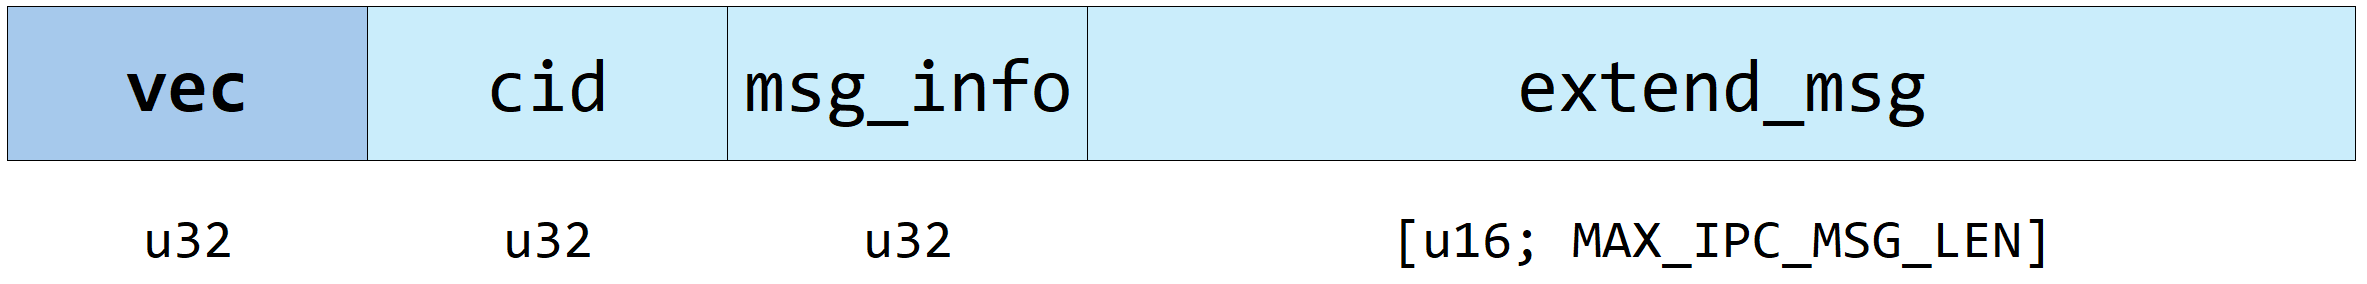
\includegraphics[width=0.8\textwidth]{images/ipc_item.png}
  \caption{ipcitem结构}\label{ipc_item结构}
\end{figure}

\subsection{环形队列结构优化}

依据\ref{sec:buffer}中的设计,缓冲区实现如图\ref{缓冲区类图}所示。

\begin{figure}[htbp]
  \centering
  \includesvg[inkscapelatex=false,width=\textwidth]{images/newbuffer}
  \caption{缓冲区类图}\label{缓冲区类图}
\end{figure}

缓冲区中\texttt{data}为数据区,由长度为4096的\texttt{ipc\_item}数组实现,用于存储调用时的传递消息。

\texttt{req\_items}和\texttt{res\_items}分别为请求消息与回复消息的索引队列,两者均采用\texttt{ItemsIdxQueue}数据结构实现。\texttt{ItemsIdxQueue}基于\texttt{SafeRingBuffer}封装,实现了一个线程安全的环形队列,提供了入队\texttt{write\_free\_idx}和出队\texttt{get\_first\_idx}两个基础方法。
\texttt{SafeRingBuffer}是一个无锁环形缓冲区,其内部使用原子变量\texttt{count}记录缓冲区中有效元素的数量,以此保证安全的读写。

\texttt{recv\_req\_status}和\texttt{recv\_reply\_status}为两个布尔类型的原子变量,分别表示接受请求的协程的当前状态与接受回复的\texttt{dispatcher}协程的当前状态。这两个状态标志减少了唤醒的次数,避免了重复调度。

\texttt{idx\_allocator}为数据区存储空间的索引分配器,负责管理数据区索引号的分配与回收,其内部同样使用位图实现。

缓冲区索引号的分配仅由用户态线程发起,而内核中的处理协程始终使用相同的索引号进行回复。因此,缓冲区的索引号总是由同一线程进行分配,具有天然的线程安全性。同时,两个环形队列的通过原子变量实现了并发访问控制,整个缓冲区在多线程环境下可实现无锁并发访问。该设计降低了因分配器引入导致的性能开销,使分配回收操作在极短的时间内即可完成,确保了高并发场景下的稳定性与效率。

\section{执行器的TAIC适配}

为了使异步运行时能够调用硬件能力,本设计对内核中异步运行时的执行器\texttt{Executor}中部分数据结构与方法进行了重写。

因为缓冲区的逻辑优化,已不再需要进行消息转发,因此本设计删除了相关变量,并将原有的就绪队列改为TAIC中队列的Arc引用\texttt{Arc<LocalQueue>}。在异步运行时初始化时,会调用下层的接口层代码,申请一个就绪队列,并将其引用传给执行器完成就绪队列的初始化。

\texttt{spawn}为执行器的协程生成方法。在该方法中,\texttt{Executor}使用TAIC提供的\texttt{task\_enqueue}方法将生成的协程加入就绪队列。因为TAIC句柄的第一位和第二位用作重复注册和抢占的标志位,因此调用该方法时需要协程id左移2位。

\texttt{fetch}为执行器从就绪队列中调度协程执行的方法。在该方法中使用TAIC提供的\texttt{task\_dequeue}方法取出就绪队列中的就绪协程。


\section{异步系统调用注册}

为实现上述修改,本设计修改了原有的异步系统调用注册相关代码。原有的实现中,异步系统调用注册时会对注册方的相关能力进行检查,并根据调用方生成一个用于处理异步系统调用的协程。本设计中删除了用户态中断的部分逻辑,增加了生成协程时硬件能力注册的代码。


\section{用户接口封装}

\subsection{进程初始化}

为使用户态进程支持异步系统调用能力,系统需要在创建进程时准备相关数据结构,完成异步系统调用的初始化。

\begin{figure}[htbp]
  \centering
  \includesvg[inkscapelatex=false,width=\textwidth]{images/initsyscall}
  \caption{线程初始化异步系统调用时序图}\label{initsyscall}
\end{figure}

该过程时序如图\ref{initsyscall}所示。系统首先需要对异步运行时进行初始化,然后对初始化TAIC的硬件能力。再此过程中,会将TAIC的读写寄存器映射到用户态地址空间。然后对该进程分配接受内核回复通知的能力。基于该通知,利用TAIC的\texttt{alloc\_receiver}函数为进程分配一个队列。接着会为进程初始化一个异步通信的缓冲区,将该缓冲区注册用于异步系统调用,并访问缓冲区的能力。然后,基于通知能力,进行系统调用,进行3.2所述的异步系统调用注册。在注册成功后,利用接口层的\texttt{register\_sender}函数,将当前进程的TAIC队列注册成为系统内核全局队列信号的发送者。最后,调用异步运行时的接口,生产用于中断向量不足时间接唤醒的分发协程。


\subsection{异步系统调用发送协程}

使用该系统的用户可利用异步运行时,生成协程发起异步系统调用。目前给出可能的协程内进行异步系统调用的方法。

协程首先应调用结构层的\texttt{alloc\_vec}函数尝试申请分配一个vec。若分配成功,则利用该vec,调用\texttt{register\_receiver}注册函数将本协程注册成消息的接受者。然后即可通过异步系统调用接口进行异步系统调用。在调用完成后,应释放分配的vec。

该部分算法伪代码如算法\ref{alg:client_call}:

\begin{algorithm}
  \caption{Client Async SysCall}\label{alg:client_call}
  \begin{algorithmic}
    \Procedure{client\_call\_test}{sender\_id, msg}
    \State \textbf{unsafe}
    \State $cid \gets$ \Call{coroutine\_get\_current}{}
    \State $vec \gets$
    \If {\Call{alloc\_vec}{} \textbf{returns} Some($res$)}
    \State \Call{register\_receiver}{sender\_id, res, cid, true, true}
    \State $res$
    \Else
    \State $0$
    \EndIf
    \For {$i = 0$ \textbf{to} ${call\_cnt} - 1$}
    \State $reply \gets$ \Call{riscv\_Page\_Map}{vec, args} \Comment{await}
    \If {$reply$ \textbf{is Ok}}
    \State \Call{cope}{$reply$}
    \Else
    \State \Call{panic}{``client test fail!''}
    \EndIf
    \EndFor
    \State \Call{free\_vec}{vec}
    \EndProcedure
  \end{algorithmic}
\end{algorithm}


\subsection{异步系统调用接口}

为方便用户使用异步系统调用,异步库提供异步系统调用接口,异步系统调用进行封装。该类接口中会对参数进行编码转换,构造成异步系统调用消息。最后调用\ref{sec:asynccallfunc}中的异步call函数进行异步调用。ReL4中异步系统调用的接口函数如表\ref{syscalltable}所示。

\begin{table}[htb]
  \centering
  \caption{ReL4 异步系统调用表}\label{syscalltable}
  \begin{tabular}{@{}ll@{}}
    \toprule
    \textbf{系统调用}                               & \textbf{功能描述}                  \\
    \midrule
    \texttt{syscall\_untyped\_retype}           & 将未初始化对象重新类型化为指定内核对象类型。         \\
    \texttt{syscall\_riscv\_page\_get\_address} & 获取虚拟页对应的物理地址。                  \\
    \texttt{syscall\_putchar}                   & 向控制台输出单个字符。                    \\
    \texttt{syscall\_putstring}                 & 向控制台输出字符串。                     \\
    \texttt{syscall\_tcb\_bind\_notification}   & 将通知对象绑定到指定的 TCB 上。             \\
    \texttt{syscall\_tcb\_unbind\_notification} & 从 TCB 上解绑通知对象。                 \\
    \texttt{syscall\_cnode\_copy}               & 拷贝 capability 到另一个 cnode 中。    \\
    \texttt{syscall\_cnode\_delete}             & 删除 cnode 中的 capability。        \\
    \texttt{syscall\_cnode\_mint}               & 复制并设置新的权限与 badge 的 capability。 \\
    \texttt{syscall\_riscv\_page\_map}          & 映射物理页到虚拟地址空间。                  \\
    \texttt{syscall\_riscv\_page\_unmap}        & 解除物理页的虚拟映射。                    \\
    \texttt{syscall\_riscv\_pagetable\_map}     & 映射页表到虚拟地址空间。                   \\
    \texttt{syscall\_riscv\_pagetable\_unmap}   & 解除页表映射。                        \\
    \bottomrule
  \end{tabular}
\end{table}

本设计对ReL4中原有接口的封装进行了微小改动,加入了中断向量参数的构造与传递,修改了系统调用接口的常量参数。

\subsection{异步call函数}\label{sec:asynccallfunc}

\texttt{seL4\_call\_with\_item}为发起异步系统调用的关键函数。该函数接受三个参数:接收方id,中断向量以及进程间通信条目,可对目标发起异步的\texttt{sel4\_call}调用。在接收方为0号的异步系统调用中,会调用通知对象的send能力,对系统中处理异步系统调用的端点发送消息,并等待reply回复。

该方法首先获取接受方的异步通信缓冲区,然后向缓冲区申请id。成功申请到id后,依据传入的消息参数将消息写入缓冲区。此时,会检测冲区中的原子变量\texttt{recv\_req\_status}。若原子变量为\texttt{false},则说明内核中的处理协程已经因空闲阻塞。此时会先调整原子变量的值,防止并发时重复唤醒。然后调用接口层中的\texttt{send\_signal}方法像内核发送信号,唤醒对应协程。完成操作后,该方法会在此阻塞,等待内核的回复。当协程因收到回复而被再次调度执行时,会依据先前的缓冲区id获取回复消息并进行返回。

该方法的伪代码如下所示:

\begin{algorithm}
  \caption{\texttt{sel4\_call\_with\_item(recv, vec, item)}}
  \begin{algorithmic}[0]  % 关闭行号
    \State buffer $\gets$ try get mutable buffer from \texttt{SENDER\_MAP[*recv]}
    \If{buffer is None}
    \State \Return \texttt{Err("Failed to get service buffer")} \Comment 获取失败
    \EndIf

    \State idx $\gets$ buffer.idx\_allocator.allocate()
    \If{idx is None}
    \State \Return \texttt{Err("Failed to allocate index in buffer")} \Comment 索引分配失败
    \EndIf

    \State buffer.data[idx] $\gets$ *item
    \If{buffer.req\_items.write\_free\_idx(idx) is Err}
    \State \Return \texttt{Err("Failed to write free index")} \Comment 写入请求队列失败
    \EndIf

    \If{buffer.recv\_req\_status.load() == false}
    \State buffer.recv\_req\_status.store(true)
    \State send\_signal(*recv, vec) \Comment 唤醒接收方
    \State \texttt{TEST\_TAIC\_SEND\_SIGNAL += 1}
    \EndIf

    \State yield\_now().await \Comment 阻塞等待响应
    \State buffer.idx\_allocator.release(idx) \Comment 释放索引
    \State \Return \texttt{Ok(buffer.data[idx])}
  \end{algorithmic}
\end{algorithm}

\subsection{分发协程}
当中断向量不足,需要分发协程进行唤醒的软件转发。异步库提供该协程的实现:

该协程相当于接收回复消息的服务端。协程首先会从参数中解析出异步系统调用的缓冲区,然后将自身注册成为0号中断向量的接收者,然后会进入主循环。在循环内部,该协程不断从缓冲区的“接受回复索引队列”中取出需要唤醒的消息id。如果成功取到,则会根据消息中的协程id,通过\texttt{coroutine\_wake}接口唤醒对应的协程。如果队列为空,则会调整缓冲区中表示自身状态的原子变量
\texttt{recv\_reply\_status},然后调用\texttt{yield\_now}接口阻塞自身,让出执行权。

\section{内核处理算法}

内核中异步系统调用的处理协程相当于内核中的服务端,与分发协程类似。该协程会在异步系统调用注册时生成,并通过参数传递得到缓冲区能力。协程解析出缓冲区后,即进入主循环处理消息。

在主循环中,协程尝试从缓冲区的\texttt{req\_items}索引队列中获取消息索引。如果成功获取到消息,则解析消息中的标签,根据不同的系统调用进行不同的处理。处理完成红,会根据消息索引将处理的结果写回缓冲区。如果请求消息中的中断向量为0,则直接通过硬件接口\texttt{send\_signal}发送信号唤醒原协程。否则,会先将回复消息的索引写入队列\texttt{res\_items},然后根据缓冲区中的原子变量\texttt{recv\_reply\_status}判断分发协程的状态。若分发协程已经阻塞,则通过\texttt{send\_signal}接口唤醒分发协程。

当缓冲区中所有消息都被处理完毕后,协程会调用\texttt{yield\_now}接口阻塞自身,等待唤醒。

该部分的伪代码如算法\ref*{alg:async_syscall_handler}所示:

\begin{algorithm}[h]
  \caption{异步系统调用处理协程 \texttt{async\_syscall\_handler}}\label{alg:async_syscall_handler}
\begin{algorithmic}
\Function{async\_syscall\_handler}{$process\_id$, $tcb$}
    \State $new\_buffer \gets$ \Call{convert\_to\_mut\_type\_ref}{$new\_buffer\_cap$}
    \Loop
        \If{\Call{has\_request\_item}{$new\_buffer$}}
            \State $idx \gets$ \Call{get\_first\_idx}{$new\_buffer.req\_items$}
            \State $item \gets$ \Call{deep\_copy}{$new\_buffer.data[idx]$}
            \State $label \gets$ \Call{AsyncMessageLabel::from}{$item.msg\_info$}
            \State \Call{debug}{"handle async syscall: \{label\}"}
            \State $reply \gets$ \Call{handle\_syscall}{$label$, $item$}
            \State $new\_buffer.data[idx] \gets item$
            \If{$item.vec \neq 0$}
                \State \Call{send\_signal}{$process\_id$, $item.vec$}
            \Else
                \State \Call{release\_buffer\_item}{$new\_buffer$, $idx$}
                \If{\Call{recv\_reply\_status}{$new\_buffer$} is false}
                    \State \Call{set\_recv\_reply\_status}{$new\_buffer$, true}
                    \State \Call{send\_signal}{$process\_id$, 0}
                \EndIf
            \EndIf
        \Else
            \State \Call{set\_recv\_req\_status}{$new\_buffer$, false}
            \State \Call{yield\_now}{} \Comment{Block until next notification}
        \EndIf
    \EndLoop
\EndFunction
\end{algorithmic}
\end{algorithm}



\section{本章小结}

本章详细介绍了支持异步系统调用的系统关键实现细节。首先,通过中断向量分配器的设计,实现了协程与硬件中断之间的高效映射,使用基于位图的分配结构以及硬件友好的算法,提升了分配性能。随后,在接口层对内核与用户态的硬件队列进行了合理封装,分别实现了局部队列的独立管理与中断驱动的异步唤醒机制。

在缓冲区部分,针对高并发场景进行了深度优化。通过双环形队列配合原子状态变量,确保了消息队列的无锁并发访问能力,同时减少了不必要的线程唤醒,有效提升了运行效率。缓冲区索引的线程安全性也通过线程唯一分配策略得以保证。

针对执行器模块,本设计完成了其与硬件异步能力的适配,替换了原有就绪队列逻辑,并引入基于TAIC队列的协程调度机制,形成软硬协同的调度执行路径。此外,为适配上述机制,对异步系统调用的注册、发起、接收、回复及中断转发等环节进行了系统性重构。

最后,完整实现了服务端处理协程与客户端分发逻辑,为异步系统调用提供了完整的数据路径和调度保障,确保异步系统调用在用户态与内核态间的高效传输与响应。通过本章的设计与实现,整个系统的异步通信能力得以构建,为后续章节的性能评估与应用部署奠定基础。
\chapter{实验与评估}

基于上述实现,本设计完成了对rel4系统中,基于TAIC的异步系统调用优化。为验证系统的功能正确性与性能优化情况,本设计编写了测试用例并FPGA上进行实验验证。本章将对实验的情况进行讲解,并对实验结果进行分析。

\section{测试环境与平台}

本实验采用的宿主机环境如下表所示:

\begin{table}[htbp]
\centering
\renewcommand{\arraystretch}{1.2}
\begin{tabular}{|l|l|}
\hline
\textbf{CPU} & AMD Ryzen 7 5800H with Radeon Graphics 3.20 GHz \\
\hline
\textbf{操作系统} & Windows 11 专业版,操作系统版本	26100.3915 \\
\hline
\textbf{系统架构} & x86\_64 \\
\hline
\textbf{内存大小} & 32 GB \\
\hline
\end{tabular}
\caption{宿主机环境配置}
\label{tab:experiment-platform}
\end{table}


本实验采用的虚拟机环境如下表所示:

\begin{table}[htbp]
\centering
\renewcommand{\arraystretch}{1.2}
\begin{tabular}{|l|l|}
\hline
虚拟机软件 & VMware® Workstation 17 Pro \\
\hline
虚拟机版本 & 17.5.0 build-22583795 \\
\hline
虚拟机操作系统 & Ubuntu 24.04.1 LTS \\
\hline
虚拟机内核版本 & Linux 6.11.0-25-generic \\
\hline
虚拟机核心数与内存大小 & 4核心,8GB \\
\hline
\end{tabular}
\caption{虚拟机环境配置}
\label{tab:vmware-platform}
\end{table}

本实验在FPGA上对异步系统调用性能进行评估验证,开发板部分信息如下:

% 表:开发板及FPGA型号信息
\begin{table}[htbp]
\centering
\renewcommand{\arraystretch}{1.2}
\begin{tabular}{|l|l|}
\hline
\textbf{开发板型号} & AXU15EG \\
\hline
\multicolumn{2}{|c|}{RISC-V系统参数} \\
\hline
核心数量 & 2核 \\
\hline
频率 & 100 MHz \\
\hline
BTB入口数量 & 40 \\
\hline
L2缓存大小 & 2 MB \\
\hline
内存大小 & 2 GB \\
\hline
\end{tabular}
\caption{FPGA 开发板基本信息}
\label{tab:fpga-info}
\end{table}

\section{功能测试}

\subsection{TAIC调用测试}

本测试用于测试将TAIC适配进系统并允许用户线程访问后,是否能正常使用全局队列的各项功能。测试模拟用户线程进行任务的入队出队操作。测试中,线程使用硬件调度器分配一个全局队列,然后将100个任务入队,再将100个任务出队。

测试结果如图\ref{taictest}所示

\begin{figure}[htbp]
  \centering
  \includegraphics[width=\textwidth]{images/TAICtest.png}
  \caption{TAIC调用测试结果}\label{taictest}
\end{figure}

由结果可知,测试成功将100个队列入队并出队,测试结果与预期相符,说明用户线程使用硬件能力正常。

\subsection{缓冲区读写测试}

本测试用于测试共享缓冲区的读写功能是否正常。测试模拟用户协程申请缓冲区索引并写入数据,内核服务协程从缓冲区读取数据并进行回复。测试时,用户协程向缓冲区写入字符串"message from usermode",内核协程拿到数据后回复"message from kernel"。

测试结果如图\ref*{buffertest}所示

\begin{figure}[htbp]
  \centering
  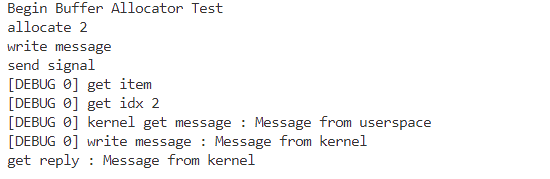
\includegraphics[width=\textwidth]{images/buffertest.png}
  \caption{缓冲区读写测试结果}\label{buffertest}
\end{figure}

由结果可知,用户协程与内核协程成功利用缓冲区进行通信,索引分配回收正常。

\subsection{异步系统调用测试}

本测试分别测试进行硬件优化后,ReL4系统中原有的各种异步系统调用功能是否正常。分别为输出类系统调用、通知类系统调用和内存映射类系统调用。

输出类系统调用测试用例如下:

\begin{enumerate}
  \item 调用 \texttt{PutChar} 异步系统调用输出一个字符 `'X'`。
        预期结果: 控制台输出字符 `'X'`,并在日志中记录系统调用被调度。

  \item 调用 \texttt{PutString} 异步系统调用输出字符串 `"11111"`。
        预期结果: 控制台输出字符串 `"11111"`,日志显示异步系统调用调度信息。
  \item 调用 \texttt{RISC-VGetPageAddress} 异步系统调用获取目标虚拟地址 \texttt{vaddr} 所在页帧的物理地址,并通过日志输出。\\
        预期结果:日志记录异步系统调用触发,并显示页帧的物理地址,物理地址应与同步调用结果一致
\end{enumerate}

\begin{figure}[htbp]
  \centering
  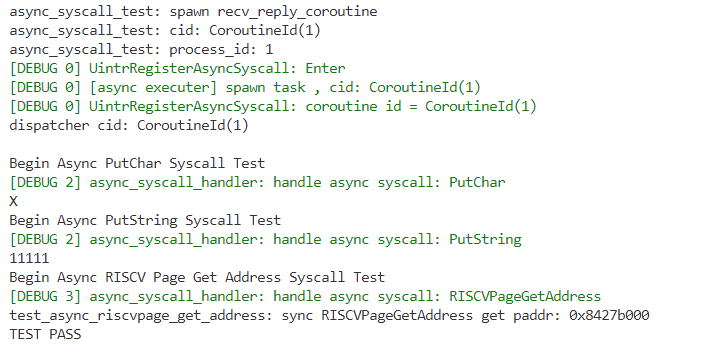
\includegraphics[width=\textwidth]{images/output_test.png}
  \caption{输出类系统调用功能测试结果}\label{outputtest}
\end{figure}

测试结果如图\ref{outputtest}所示。由结果可知,异步系统调用的输出功能正常,日志记录了异步系统调用的触发信息。测试结果与预期一致。

通知类系统调用测试用例如下:

\begin{enumerate}
  \item 调用 \texttt{TCBBindNotification}将一个通知与TCB绑定\\
        预期结果:日志记录异步系统调用触发,并显示TCB与通知地址。
  \item 调用 \texttt{TCBUnbindNotification}解除通知与TCB的绑定\\
        预期结果:日志记录异步系统调用触发,并显示TCB与通知地址。
\end{enumerate}

\begin{figure}[htbp]
  \centering
  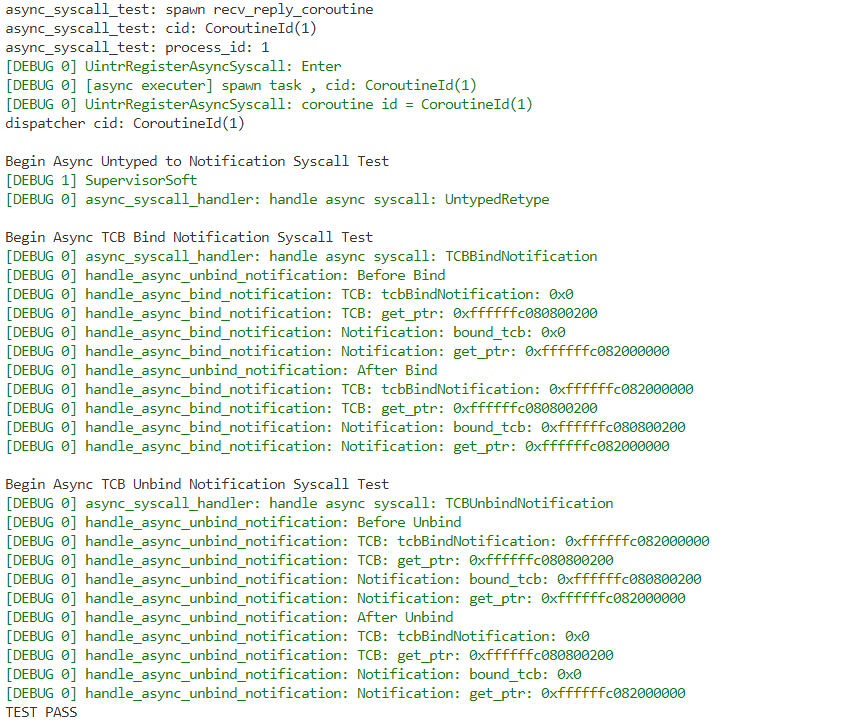
\includegraphics[width=\textwidth]{images/ntfntest.png}
  \caption{通知类系统调用功能测试结果}\label{ntfntest}
\end{figure}

测试结果如图\ref{ntfntest}所示。由结果可知,异步系统调用的通知功能正常,日志记录了异步系统调用的触发信息。测试结果与预期一致。

内存映射类系统调用测试用例如下:
\begin{enumerate}
  \item 调用 \texttt{RISC-VPageTableMap}将页表映射到虚拟地址空间。
        预期结果:日志记录异步系统调用触发,并显示相关信息。
  \item 调用 \texttt{RISC-VPagemap} 将一个物理页帧利用页表映射到虚拟地址中。
        预期结果:日志记录异步系统调用触发,并显示相关信息。
  \item 尝试在该页面读写内存。
        预期结果:成功在该页帧读写内存。
\end{enumerate}


\begin{figure}[htbp]
  \centering
  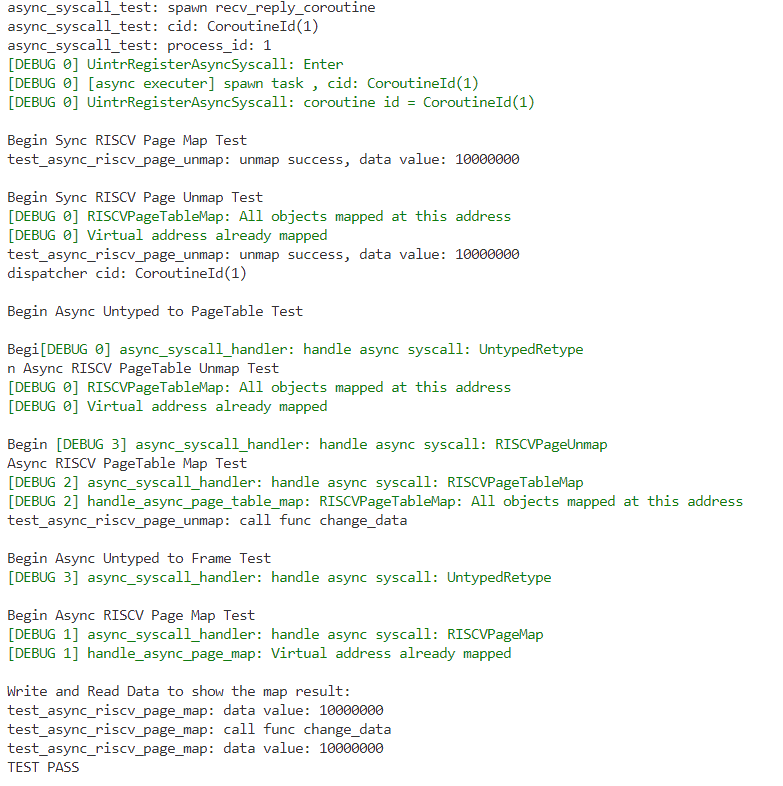
\includegraphics[width=\textwidth]{images/memtest.png}
  \caption{内存映射类系统调用功能测试结果}\label{memtest}
\end{figure}

测试结果如图\ref{memtest}所示。由结果可知,异步系统调用的内存映射功能正常,日志记录了异步系统调用的触发信息。测试结果与预期一致。

\section{性能测试}

\subsection{测试对象说明}

本实验中选取内存映射(RISC-VPageMap)与取消映射(RISC-VPageUnmap)两个系统调用作为测试对象并设计实验场景。在基于 RISC-V架构的rel4微内核操作系统中,内存空间的管理权下放至用户态程序,用户负责页表的维护与内存区域的动态分配与释放。因此,用户态程序在运行过程中必须频繁地调用 RISC-VPageMap 和 RISC-VPageUnmap,以实现对虚拟地址空间的有效控制。因此,将二者作为本实验的测试对象,可以用于评估异步系统调用的性能。

\subsection{性能测试流程}

本实验中,测试会模拟线程多次映射物理页帧与解除物理页帧的情况。映射与解除映射时分别调用异步系统调用RISC-VPageMap与RISC-VPageUnmap。测试程序首先会初始化一个线程并为其赋予内存分配能力。随后,线程生成一定数量的物理页框供测试时映射。

为表征系统在不同并发度下的性能表现,实验设置了1、2、4、8、16、32、64、128及256多组并发度。对于每个并发度,测试程序会生成对应数量的协程。每个协程对同一页框执行10轮调用操作,每轮包括一次页帧映射与解除映射。

测试分别基于现有实现和ReL4原有的实现进行,以此对比引入TAIC硬件调度器前后的性能差异。此外,为进行完整的性能评估,实验使用同步系统调用作为对照。同步测试中,使用单线程循环进行系统调用,对页框进行映射与解除映射。系统调用总次数与异步调用相同。

性能评估采用以下两个指标:

1. 平均耗时

在异步测试中,该指标为从所有协程启动运行时,到所有协程均完成系统调用后所有的总时间与系统调用次数的比值。其反应异步过程中,等效的单次用时。

在同步测试中,该指标为第一次系统调用开始,到最后一次系统调用结束所有的总时间与系统调用次数的比值。

2. 陷入频率

在测试ReL4原有实现的性能时,该指标为平均每次异步系统调用中,需要陷入内核唤醒内核中协程的次数。

在测试引入硬件调度能力后,该指标为使用硬件唤醒内核中协程的次数。


\subsection{实验结果与评估}

该性能测试结果如图\ref{性能测试结果}。

\begin{figure}[htbp]
  \centering
  \includesvg[inkscapelatex=false,width=\textwidth]{images/syscall_test}
  \caption{异步系统调用性能测试结果}\label{性能测试结果}
\end{figure}

% \begin{figure}[htbp]
%   \centering
%   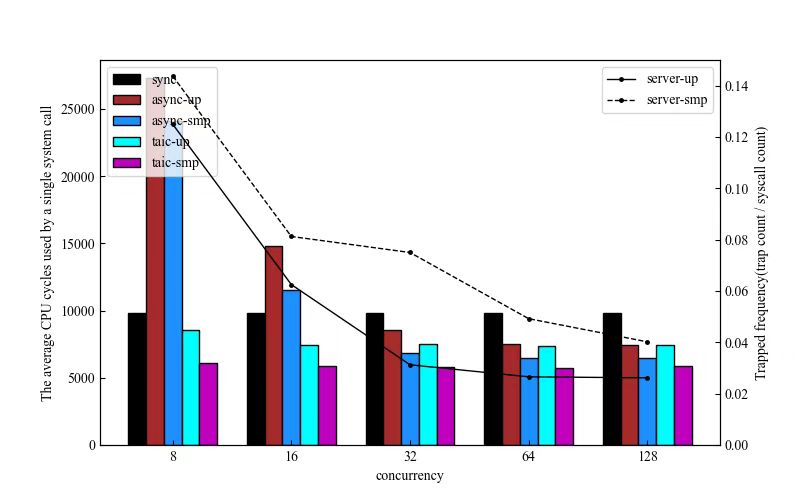
\includegraphics[width=0.8\textwidth]{images/async_syscall.jpg}
%   \caption{异步系统调用性能测试结果}\label{asyncSyscall}
% \end{figure}

\subsubsection{平均用时分析}

从结果中可以看出,在所有并发度下,使用TAIC优化后的异步系统调用平均用时均小于优化前原ReL4系统中的实现。这是由于TAIC降低了异步运行时引入所造成的开销。根据前文的分析,TAIC的使用取代了用户态中断与内核态陷入,减少了大部分原有实现中造成性能瓶颈的上下文切换。测试结果体现了优化后异步系统调用的性高效性与可用性。

由柱状图中可以看出,在并发度为4以下时,原异步实现平均用时显著高于同步,尤其在并发度为1时,单核平均用时约22000个时钟周期,约为同步调用的2倍。而优化后的异步系统调用在单核情况下耗时约为12400个时钟周期;在多核情况下耗时约7500个时钟周期,对比优化前的方案有大幅度的降低。这是由于在低并发下,原有实现中内核中的异步系统调用处理协程与用户线程中的分发协程因为没有足够数量的处理请求,大多处于空闲阻塞状态,这导致平均每次调用所需的唤醒频次较高。而TAIC硬件的使用针对这一问题进行了优化,因此在低并发下的性能有较大的提高。

随之并发度的不断增加,所有方案的平均用时均有下降趋势,但使用TAIC优化后,平均用时仍具有最低的平均用时。这是由于并发数量的增加均分了内核处理时用户协程的等待时间。但并发度4以上时,使用TAIC优化后的平均用时变化较小。这是由于并发的提高通过减少唤醒频次,减小了上下文切换的开销。引入TAIC后,取消了上下文切换的过程,因此优化后的平均用时随并发的增加变化较小。

实验结果显示,单核的测试结果高于多核的测试结果。这是由于单核情况下,系统内核与用户线程共用同一核心,即使在引入TAIC的情况下,仍采用陷入内核的方式处理,以减少响应延迟。

在并发度小于4的情况,优化后单核异步系统调用的性能仍高于同步。一方面,异步功能的引入仍具有一定的开销,低并发下缺少足够数量的并发请求来均摊异步功能所造成的额外开销。另一方面,单核情况下的内核陷入无法完全避免,因此仍具有较高的性能开销。

结果显示,多核情况下的所有平均用时均优于同步,且对比同步调用具有约25\%到30\%的平均用时减少。虽然低并发下的单核性能略高于同步,但相较ReL4原有设计已有明显改善。并发度为1的情况下,平均用时减少约40\%,且测试指标在并发为2时已与同步基本持平。因此本设计在单核情况下仍有一定的可用性。随着多核处理器的普及,单核的性能瓶颈问题将逐渐被解决。综上所述,本设计对ReL4系统在低并发情况下的异步系统调用平均用时有显著的提升并具有可用性。

\subsubsection{陷入频率分析}

图中折线图部分展示了系统调用的陷入频率。

经过对实验结果的分析可知,不论在单核还是多核的测试环境下,采用优化后的异步系统调用模型的陷入频率均呈现出随着并发度提升而持续下降的趋势。如图中所示,在单核环境下,异步系统调用的陷入频率从初始并发度1开始,逐步下降至并发度32时的0.08;而在多核环境下该频率与单核变化趋势类似,但在并发度大于8时较单核略有提高。

造成这一现象的主要原因是,随着并发度的增加,用户态线程发起系统调用的整体速率提高,导致内核中协程的处理量增加。内核中的处理协程进入较长时间的持续运行状态,使得大多数系统调用请求可以被协程直接响应,无需阻塞或等待唤醒,从而显著减少了主动唤醒的次数。

\section{两种中断注册机制的对比}\label{sec:regintctest}

为验证TAIC两种注册机制对异步性能的影响,本实验为两种实现方式进行了对比实验,分别测试在一次性注册与持续性注册下异步系统调用的平均用时。

测试结果如图\ref{中断向量注册机制对比测试结果}。

\begin{figure}[htbp]
  \centering
  \includesvg[inkscapelatex=false,width=0.8\textwidth]{images/taiccompare}
  \caption{中断向量注册机制对比测试结果}\label{中断向量注册机制对比测试结果}
\end{figure}

实验结果显示,两种中断注册机制在系统调用性能方面存在显著差异,其中持续性注册机制在所有并发条件下均表现出更优的性能。特别是在高并发环境下,持续性注册机制的优势更加明显,其平均系统调用用时显著低于单次注册机制。

随着并发度的提升,单次注册机制的平均调用用时呈现持续上升趋势,而持续性注册机制逐渐减小,在并发度4以上时,单次注册机制的平均系统调用延迟迅速上升,远高于持续性注册方式。

造成此现象的原因是,两种机制对taic中接受方注册的方式不同。单次注册机制在每次阻塞前均注册一次信号接收。这种实现虽然较为通用,但为了避免内核与用户态线程同时读写硬件寄存器而造成冲突,硬件接口层需对相关函数添加互斥锁进行保护。该互斥锁在低并发下影响较低,但在高并发场景中有较显著的性能影响。随着并发线程数的增加,频繁的争用互斥锁会导致CPU大部分时间在无意义的等待中。

而持续性注册机制在异步系统调用注册时就完成了接收方的注册,并保持注册状态。该方法下整个线程运行期间,内核无需再次进行注册操作,省去了互斥锁操作的时间成本。该机制避免了高并发情况下的冲突问题,使得优化后的异步运行时在高并发下仍有较低开销。

综上所述,在本设计中,持续性中断注册机制具有更好的性能表现,尤其在高并发场景下优势更为明显。因此,本设计最终采用持续性注册机制作为默认实现,以充分发挥硬件调度器在异步系统调用中的优势。

\section{本章小结}

本章围绕基于TAIC优化的异步系统调用机制,详细介绍了功能测试与性能评估的全过程。功能测试表明,各类异步系统调用在引入硬件调度能力后均能正确运行。性能测试结果则显示,TAIC优化在不同并发度下均有效降低了系统调用的平均用时和陷入频率,尤其在低并发和多核场景中优势显著,相较原有ReL4系统具有明显性能提升。此外,通过对比不同中断注册机制的测试结果,也进一步验证了持续性注册在特定场景下的性能优势。


% 后置内容
\backmatter

% 结论:在相应 TeX 文件撰写
% \begin{conclusion}

本文聚焦于Rel4系统在低并发场景下异步系统调用性能不足的问题,提出并实现了一种基于任务感知中断控制器(Task-Aware Interrupt Controller, TAIC)的优化方案。通过对ReL4系统进行分析并采取针对性的优化,本设计取得了以下创新性成果:

首先,本设计并实现了基于TAIC的异步系统调用路径重构。为突破ReL4中异步系统调用在用户态与内核态频繁切换导致的低并发性能劣势,本设计引入任务感知中断控制器(TAIC)作为硬件调度支持,通过改造异步运行时,将异步系统调用的任务唤醒与消息传递过程部分下沉至硬件,实现了一种无需陷入内核的异步系统调用。该系统调用路径在多核场景中完全避免了陷入带来的上下文切换开销。实验表明,该机制在多核低并发情况下平均延迟下降超过60\%,在不引入同步路径的前提下兼顾了“微内核最小化”与“高效异步通信”的设计原则。

其次,本文实现了面向高并发调度的中断资源动态分配机制。面对TAIC仅支持有限数量硬件中断向量的约束,本设计创新性地提出中断向量“动态映射+调度复用”策略。在硬件资源充足时,实现一对一直接唤醒;当资源不足时,引入dispatcher协程实现协程间接唤醒,从而实现硬件资源复用与调度效率的兼顾。同时本文还构建了一个中断向量位图管理器,在接口层实现高效资源分配与释放机制。该机制适用于动态并发度变化的异步场景,是软硬协同调度机制的重要尝试。

最后,本设计提出了结构化异步缓冲区与无锁访问设计。为进一步适配硬件调度模型,本文对原有基于环形队列的缓冲区结构进行了深度重构。新设计采用“消息槽+索引队列”的双结构体系,支持消息乱序处理与并发访问,结合原子变量实现线程间状态同步,构建了支持多协程并发写入、内核协程无锁读取的共享通信缓冲区。

本设计通过引入硬件优化协程调度、重构异步系统调用路径、优化缓冲区结构及调度机制,有效减少了上下文切换的频率并提高了系统在多种并发度下的性能表现。全文的研究和实验结果表明,该方案在性能层面均取得了显著提升,具有较强的工程实用价值和理论指导意义。

尽管本文在Rel4系统基础上初步完成了异步系统调用的优化设计与验证,但仍有若干方向值得进一步深入研究与探索:

首先,可以尝试将内核中的任务整体进行异步化改造,结合TAIC的硬件调度能力,可完全避免异步系统调用在单核情况下的上下文切换,进一步提升系统在单核环境下的响应效率。其次,目前本设计的优化方案仅基于risc-v平台完成初步集成与性能验证,后续可考虑将本系统移植至多种硬件平台,从而提升方案的通用性与平台适应能力。最后,可尝试将本系统集成至典型的应用系统,基于实际业务请求的性能评估与长期稳定性测试,从而全面评估该优化方案在实际应用场景下的可行性与稳定性。

\end{conclusion}

% 参考文献:
% 添加文献时,请按 BibTeX 格式添加至 misc/ref.bib,并在正文所需位置使用 \cite{…} 引用。
% 如无特殊需要,无需改动相应 TeX 文件。
% %%
% The BIThesis Template for Bachelor Graduation Thesis
%
% 北京理工大学毕业设计(论文)参考文献 —— 使用 XeLaTeX 编译
%
% Copyright 2020-2023 BITNP
%
% This work may be distributed and/or modified under the
% conditions of the LaTeX Project Public License, either version 1.3
% of this license or (at your option) any later version.
% The latest version of this license is in
%   https://www.latex-project.org/lppl.txt
% and version 1.3 or later is part of all distributions of LaTeX
% version 2005/12/01 or later.
%
% This work has the LPPL maintenance status `maintained'.
%
% The Current Maintainer of this work is Feng Kaiyu.
%
% Compile with: xelatex -> biber -> xelatex -> xelatex
%
% 如无特殊需要,本页面无需更改

\begin{bibprint}

\printbibliography[heading=none]

\end{bibprint}

% 附录:在相应 TeX 文件撰写;不需要时可删除
% %%
% The BIThesis Template for Bachelor Graduation Thesis
%
% 北京理工大学毕业设计(论文)附录 —— 使用 XeLaTeX 编译
%
% Copyright 2020-2023 BITNP
%
% This work may be distributed and/or modified under the
% conditions of the LaTeX Project Public License, either version 1.3
% of this license or (at your option) any later version.
% The latest version of this license is in
%   https://www.latex-project.org/lppl.txt
% and version 1.3 or later is part of all distributions of LaTeX
% version 2005/12/01 or later.
%
% This work has the LPPL maintenance status `maintained'.
%
% The Current Maintainer of this work is Feng Kaiyu.
%
% Compile with: xelatex -> biber -> xelatex -> xelatex

\begin{appendices}
  附录相关内容…

  % 这里示范一下添加多个附录的方法:
  % 使用 \section 来添加一个附录

  \section{\LaTeX 环境的安装}
  \LaTeX 环境的安装。

  \section{BIThesis 使用说明}
  BIThesis 使用说明。

  \textcolor{blue}{附录是毕业设计(论文)主体的补充项目,为了体现整篇文章的完整性,写入正文又可能有损于论文的条理性、逻辑性和精炼性,这些材料可以写入附录段,但对于每一篇文章并不是必须的。附录依次用大写正体英文字母 A、B、C……编序号,如附录 A、附录 B。阅后删除此段。}

  \textcolor{blue}{附录正文样式与文章正文相同:宋体、小四;行距:22 磅;间距段前段后均为 0 行。阅后删除此段。}

\end{appendices}

% 致谢:在相应 TeX 文件撰写
% %%
% The BIThesis Template for Bachelor Graduation Thesis
%
% 北京理工大学毕业设计(论文)致谢 —— 使用 XeLaTeX 编译
%
% Copyright 2020-2023 BITNP
%
% This work may be distributed and/or modified under the
% conditions of the LaTeX Project Public License, either version 1.3
% of this license or (at your option) any later version.
% The latest version of this license is in
%   https://www.latex-project.org/lppl.txt
% and version 1.3 or later is part of all distributions of LaTeX
% version 2005/12/01 or later.
%
% This work has the LPPL maintenance status `maintained'.
%
% The Current Maintainer of this work is Feng Kaiyu.
%
% Compile with: xelatex -> biber -> xelatex -> xelatex

% 致谢部分尽量不使用 \subsection 二级标题,只使用 \section 一级标题
\begin{acknowledgements}
  值此论文完成之际,首先向我的导师……

  \textcolor{blue}{致谢正文样式与文章正文相同:宋体、小四;行距:22 磅;间距段前段后均为 0 行。阅后删除此段。}
\end{acknowledgements}


\end{document}
